\documentclass[a4paper,12pt]{article}

\usepackage[utf8]{inputenc}
\usepackage[T2A]{fontenc}
\usepackage[russian]{babel}
\usepackage{amsmath,amssymb}
\usepackage{graphicx}
\usepackage{booktabs}
\usepackage{geometry}
\usepackage{hyperref}
\usepackage{float}
\usepackage{verbatim}

\geometry{margin=2cm}

\title{Пояснительная записка к проекту\\[0.3em]
\large Что именно сделано, что значат статьи, что считает Python и как это рассказывать}
\author{}
\date{11 марта 2026 года}

\begin{document}

\maketitle
\tableofcontents

\section{Зачем нужен этот PDF}
Этот файл не для сдачи преподавателю, а для меня самого. Его цель --- чтобы я мог открыть один PDF\footnote{PDF --- формат электронного документа Portable Document Format.} и быстро понять:
\begin{itemize}
    \item о чем вообще мой проект;
    \item что говорят три статьи;
    \item какие именно данные я взял;
    \item что делает Python-файл шаг за шагом;
    \item что означают таблицы и графики;
    \item что говорить на защите простыми словами.
\end{itemize}

\section{Проект в одном абзаце}
Мой проект посвящен связи между курсом EUR/USD\footnote{EUR/USD --- валютная пара ``евро к доллару США'', то есть сколько долларов дают за 1 евро.} и ценой нефти Brent\footnote{Brent --- один из основных мировых эталонных сортов нефти, по которому часто ориентируются цены на рынке.}. Идея такая: если рост нефти часто сопровождается ослаблением доллара, то это должно отражаться в росте EUR/USD. Я проверяю эту идею на воспроизводимых данных FRED\footnote{FRED --- открытая база макроэкономических и финансовых данных Federal Reserve Bank of St. Louis.}. Для короткого горизонта я смотрю дневные доходности и строю регрессию, а для длинного горизонта смотрю месячные данные, проверяю коинтеграцию\footnote{Коинтеграция --- ситуация, когда сами ряды нестационарны, но между ними существует устойчивое долгосрочное соотношение.} и оцениваю ECM\footnote{ECM, Error Correction Model --- модель исправления ошибок, которая сочетает краткосрочную динамику с возвратом к долгосрочному равновесию.}. Главный вывод: краткосрочная положительная связь есть, но после 2022 года она заметно ослабевает; очень сильной и стабильной долгосрочной связи данные не подтверждают.

\section{Что именно говорят статьи}

\subsection{Статья 1: Benlaria et al. (2020)}
\textbf{Название:} \textit{The Relationship between Crude Oil Prices, EUR/USD Exchange Rate and Gold Prices}.

\textbf{Что они делают.}
Авторы берут месячные данные с января 1999 года по октябрь 2019 года и оценивают связь между нефтью, EUR/USD и золотом через ARDL\footnote{ARDL, Auto-Regressive Distributed Lag --- модель, где текущая переменная объясняется собственными лагами и лагами других переменных.}.

\textbf{Главная идея статьи.}
Связь между переменными есть, но она проявляется в первую очередь в краткосрочной динамике. Кроме того, они пишут про однонаправленную причинность от EUR/USD к нефти.

\textbf{Что я взял из этой статьи в свой проект.}
\begin{itemize}
    \item сам вопрос ``есть ли связь между нефтью и EUR/USD?'';
    \item идею разделять краткосрочную и долгосрочную динамику;
    \item идею использовать месячную постановку для long-run части.
\end{itemize}

\subsection{Статья 2: Fratzscher, Schneider, Van Robays (2014)}
\textbf{Название:} \textit{Oil Prices, Exchange Rates and Asset Prices}.

\textbf{Что они делают.}
Авторы из ЕЦБ\footnote{ЕЦБ --- Европейский центральный банк.} смотрят на нефть, доллар и другие финансовые активы как на части единой системы финансового рынка.

\textbf{Главная идея статьи.}
Связь нефти и доллара усилилась с начала 2000-х, причем она меняется по режимам рынка. Это очень важная мысль: связь может быть не постоянной.

\textbf{Что я взял из этой статьи в свой проект.}
\begin{itemize}
    \item идею, что связь нельзя считать фиксированной;
    \item идею проверить смену режима;
    \item поэтому я отдельно сравнил период до 2022 года и период после 2022 года.
\end{itemize}

\subsection{Статья 3: Dias et al. (2025)}
\textbf{Название:} \textit{The Influence of the International Oil Price on the EUR/USD Exchange Rate}.

\textbf{Что они делают.}
Они исследуют более свежий период 2022--2024 и рассматривают влияние Brent и нефтяной волатильности\footnote{Волатильность --- мера изменчивости цены; чем она выше, тем сильнее цена колеблется.} на несколько валютных пар.

\textbf{Главная идея статьи.}
Для EUR/USD связь с нефтяным фактором не исчезает совсем, но уже не выглядит простой, изолированной и постоянной. На валюту одновременно действуют и другие глобальные факторы.

\textbf{Что я взял из этой статьи в свой проект.}
\begin{itemize}
    \item аргумент, почему важно отдельно смотреть свежие данные;
    \item понимание, что после 2022 года эффект мог ослабнуть;
    \item осторожную интерпретацию: нефть --- это фактор, но не единственный драйвер EUR/USD.
\end{itemize}

\subsection{Как три статьи соединились в мой проект}
По сути я сделал такую сборку:
\begin{itemize}
    \item из первой статьи взял базовую постановку ``нефть и EUR/USD'';
    \item из второй --- идею смены рыночных режимов;
    \item из третьей --- мотивацию внимательно посмотреть на свежий период после 2022 года.
\end{itemize}

\section{Какие данные я использовал и почему}
Я не использовал закрытые базы и не скачивал данные руками с сайтов. Вместо этого я взял открытые ряды FRED, чтобы проект был полностью воспроизводим\footnote{Воспроизводимый проект --- такой, где другой человек может заново получить те же результаты по коду и данным.}.

\begin{itemize}
    \item \texttt{DEXUSEU} --- USD за 1 EUR, то есть EUR/USD в долларовом выражении;
    \item \texttt{DCOILBRENTEU} --- цена Brent в долларах за баррель.
\end{itemize}

\textbf{Почему это хороший выбор.}
\begin{itemize}
    \item данные официальные и легко перепроверяются;
    \item их можно тянуть из Python одной строкой;
    \item это сразу делает проект аккуратным: любой человек может пересчитать результаты.
\end{itemize}

\textbf{Какие горизонты я использовал.}
\begin{itemize}
    \item дневные данные --- для краткосрочной связи;
    \item месячные данные --- для долгосрочной связи.
\end{itemize}

\textbf{Почему я беру логарифмы и доходности.}
Потому что уровни финансовых рядов часто нестационарны\footnote{Нестационарный ряд --- ряд, у которого средний уровень, разброс или зависимость от прошлого меняются со временем.}. Если строить регрессию прямо по уровням без проверки, легко получить ложную связь. Поэтому:
\[
e_t=\ln(\text{EUR/USD}_t), \qquad o_t=\ln(\text{Brent}_t),
\]
\[
\Delta e_t=e_t-e_{t-1}, \qquad \Delta o_t=o_t-o_{t-1}.
\]
Идея простая: краткосрочную динамику лучше изучать по изменениям, а не по самим уровням.

\section{Что делает Python-файл}
Вся вычислительная часть лежит в файле \texttt{src/analysis.py}. Ниже объяснение человеческим языком.

\subsection{Блок импортов}
В начале подключаются библиотеки\footnote{Библиотека в Python --- готовый набор функций и инструментов для определенных задач.}:
\begin{itemize}
    \item \texttt{pandas} и \texttt{numpy} --- для таблиц и расчетов;
    \item \texttt{matplotlib} --- для графиков;
    \item \texttt{statsmodels} --- для регрессий и эконометрических тестов\footnote{Эконометрический тест --- формальная статистическая процедура для проверки гипотез о данных и модели.};
    \item \texttt{json}\footnote{JSON --- текстовый формат хранения структурированных данных.} и \texttt{pathlib} --- для сохранения результатов и работы с путями.
\end{itemize}

\subsection{Папки проекта}
В коде задаются пути:
\begin{verbatim}
ROOT = Path(__file__).resolve().parents[1]
DATA_DIR = ROOT / "data"
RESULTS_DIR = ROOT / "results"
\end{verbatim}
То есть код знает, где хранить скачанные данные и куда складывать таблицы и графики.

\subsection{Функция \texttt{fetch\_series}}
Эта функция берет один ряд с FRED:
\begin{itemize}
    \item формирует ссылку;
    \item читает CSV;
    \item приводит дату к нормальному формату;
    \item переводит значения в числа.
\end{itemize}

Именно за счет этой функции проект воспроизводим: не нужно вручную искать файлы, все скачивается автоматически.

\subsection{Функция \texttt{write\_latex\_table}}
Она нужна только для удобства отчета. Python считает таблицы, а потом сохраняет их в виде \texttt{.tex}, чтобы их можно было вставить в LaTeX\footnote{LaTeX --- система для набора научных и учебных текстов с формулами и таблицами.} через \verb|\input{}|.

\subsection{Функция \texttt{fit\_daily\_regression}}
Это уже суть краткосрочной модели. Она оценивает регрессию
\[
\Delta e_t=\alpha+\beta_0\Delta o_t+\beta_1\Delta o_{t-1}+\gamma\Delta e_{t-1}+\varepsilon_t.
\]

\textbf{Что означают переменные.}
\begin{itemize}
    \item \texttt{r\_brent} --- текущая лог-доходность нефти;
    \item \texttt{r\_brent\_l1} --- лаг нефти;
    \item \texttt{r\_eurusd\_l1} --- лаг валютной доходности.
\end{itemize}

\textbf{Почему в коде HAC-ошибки.}
Потому что на финансовых данных обычные стандартные ошибки часто недооценивают реальную неопределенность. HAC\footnote{HAC, Heteroskedasticity and Autocorrelation Consistent --- способ корректировки стандартных ошибок, устойчивый к неодинаковой дисперсии и автокорреляции остатков.} делает выводы аккуратнее.

\subsection{Что делает \texttt{main()} по шагам}
\textbf{Шаг 1.} Создает папки \texttt{data/} и \texttt{results/}.

\textbf{Шаг 2.} Скачивает два ряда с FRED и сохраняет:
\begin{itemize}
    \item \texttt{data/eurusd\_daily.csv}
    \item \texttt{data/brent\_daily.csv}
\end{itemize}

\textbf{Шаг 3.} Объединяет ряды по датам.

\textbf{Шаг 4.} Строит:
\begin{itemize}
    \item логарифмы уровней;
    \item дневные лог-доходности;
    \item 252-дневную скользящую корреляцию.
\end{itemize}

\textbf{Шаг 5.} Переходит к месячным данным:
\begin{itemize}
    \item берет месячные средние;
    \item считает логарифмы;
    \item считает месячные доходности.
\end{itemize}

\textbf{Шаг 6.} Считает описательную статистику и ADF-тесты.

\textbf{Шаг 7.} Оценивает дневные регрессии:
\begin{itemize}
    \item на полной выборке;
    \item на периоде до 2022 года;
    \item на периоде после 2022 года.
\end{itemize}

\textbf{Шаг 8.} Проверяет коинтеграцию на месячных данных.

\textbf{Шаг 9.} Если смотреть на период 1999--2021, оценивает долгосрочную регрессию и ECM.

\textbf{Шаг 10.} Считает тесты Грейнджера.

\textbf{Шаг 11.} Строит графики:
\begin{itemize}
    \item \texttt{normalized\_levels.png}
    \item \texttt{rolling\_correlation.png}
    \item \texttt{scatter\_daily.png}
\end{itemize}

\textbf{Шаг 12.} Сохраняет ключевые числа в \texttt{key\_metrics.json} и текстовую выжимку в \texttt{analysis\_summary.txt}.

\section{Что лежит в папках и зачем}

\subsection{\texttt{data/}}
Это не ``мусор'', а основа воспроизводимости.
\begin{itemize}
    \item \texttt{eurusd\_daily.csv}, \texttt{brent\_daily.csv} --- сырые загруженные ряды;
    \item \texttt{merged\_daily.csv} --- совместная дневная выборка;
    \item \texttt{merged\_monthly.csv} --- месячная выборка.
\end{itemize}

\subsection{\texttt{results/}}
Это фактически ``кухня'' отчета. Здесь лежат:
\begin{itemize}
    \item численные таблицы в \texttt{csv}\footnote{CSV --- простой текстовый формат таблиц, где значения разделены запятыми.};
    \item те же таблицы в \texttt{tex};
    \item графики;
    \item файл \texttt{key\_metrics.json} с итоговыми числами.
\end{itemize}

\subsection{Главные файлы верхнего уровня}
\begin{itemize}
    \item \texttt{report.tex} и \texttt{report.pdf} --- основной сданный отчет;
    \item \texttt{slides.tex} и \texttt{slides.pdf} --- презентация;
    \item \texttt{speech\_notes.md} --- краткий текст устного выступления;
    \item \texttt{guide.tex} и \texttt{guide.pdf} --- этот объясняющий документ.
\end{itemize}

\section{Как читать результаты}

\subsection{Описательная статистика}
\begin{center}
\begin{tabular}{lrrrrr}
\toprule
series & mean & std & min & max & obs \\
\midrule
EUR/USD daily log return & 0.0000 & 0.0058 & -0.0300 & 0.0462 & 6468 \\
Brent daily log return & 0.0002 & 0.0263 & -0.6437 & 0.4120 & 6468 \\
\bottomrule
\end{tabular}

\end{center}

Здесь надо говорить просто: нефть намного более волатильна, чем EUR/USD. Это нормально и ожидаемо.

\subsection{ADF-тесты}
\begin{center}
\begin{tabular}{llrr}
\toprule
series & sample & adf\_stat & p\_value \\
\midrule
log EUR/USD level & 1999-01 to latest complete month & -1.9384 & 0.3142 \\
log Brent level & 1999-01 to latest complete month & -2.8872 & 0.0469 \\
EUR/USD log return & 1999-02 to latest complete month & -11.5380 & 0.0000 \\
Brent log return & 1999-02 to latest complete month & -12.7130 & 0.0000 \\
\bottomrule
\end{tabular}

\end{center}

Как это объяснять:
\begin{itemize}
    \item уровни рядов нельзя бездумно регрессировать друг на друга;
    \item доходности уже стационарны;
    \item значит, краткосрочную модель я строю корректно.
\end{itemize}

ADF\footnote{ADF, Augmented Dickey-Fuller test --- тест на наличие единичного корня, то есть на нестационарность временного ряда.} здесь нужен именно для проверки стационарности.

\subsection{Дневная регрессия}
\begin{center}
\resizebox{\textwidth}{!}{\begin{tabular}{lrrrrrrrrr}
\toprule
sample & obs & beta\_current\_oil & p\_current\_oil & beta\_lagged\_oil & p\_lagged\_oil & beta\_fx\_lag & p\_fx\_lag & r\_squared & corr\_oil\_fx \\
\midrule
Full sample (2010-01-04 to latest) & 3983.0000 & 0.0141 & 0.0057 & 0.0031 & 0.3288 & 0.0210 & 0.2135 & 0.0058 & 0.0712 \\
Pre-2022 sample & 2966.0000 & 0.0162 & 0.0094 & 0.0012 & 0.7494 & 0.0280 & 0.1427 & 0.0080 & 0.0847 \\
2022+ sample & 1016.0000 & 0.0039 & 0.7088 & 0.0119 & 0.0795 & -0.0037 & 0.9177 & 0.0033 & 0.0202 \\
\bottomrule
\end{tabular}
}
\end{center}

Это одна из самых важных таблиц.

\textbf{Что из нее надо вынести.}
\begin{itemize}
    \item На полной выборке коэффициент при текущей доходности нефти положителен и значим.
    \item До 2022 года он даже чуть сильнее.
    \item После 2022 года он почти исчезает статистически.
\end{itemize}

Простыми словами: раньше нефть лучше объясняла EUR/USD, а в последние годы связь стала слабее.

\subsection{Коинтеграция}
\begin{center}
\begin{tabular}{lrrr}
\toprule
sample & obs & coint\_stat & p\_value \\
\midrule
1999-2021 & 275 & -3.0217 & 0.1051 \\
2022-latest & 50 & -1.9465 & 0.5563 \\
Full monthly sample & 325 & -2.6277 & 0.2266 \\
\bottomrule
\end{tabular}

\end{center}

Что говорить:
\begin{itemize}
    \item на старом периоде есть только пограничный намек на долгосрочную связь;
    \item после 2022 года долгосрочная связь уже не подтверждается;
    \item поэтому основной надежный результат у меня именно краткосрочный.
\end{itemize}

\subsection{ECM}
\begin{center}
\begin{tabular}{lrrr}
\toprule
variable & coef & std\_err & p\_value \\
\midrule
const & -0.0002 & 0.0013 & 0.8949 \\
d\_brent & 0.0363 & 0.0149 & 0.0148 \\
d\_brent\_l1 & 0.0039 & 0.0127 & 0.7587 \\
d\_eurusd\_l1 & 0.2859 & 0.0550 & 0.0000 \\
ecm\_l1 & -0.0300 & 0.0166 & 0.0714 \\
\bottomrule
\end{tabular}

\end{center}

Как объяснять:
\begin{itemize}
    \item текущий нефтяной фактор положительно влияет на месячное изменение EUR/USD;
    \item коэффициент коррекции ошибки отрицательный, то есть знак правильный;
    \item но статистическая значимость пограничная, поэтому я не делаю слишком сильных заявлений.
\end{itemize}

\subsection{Графики}
\begin{figure}[H]
\centering
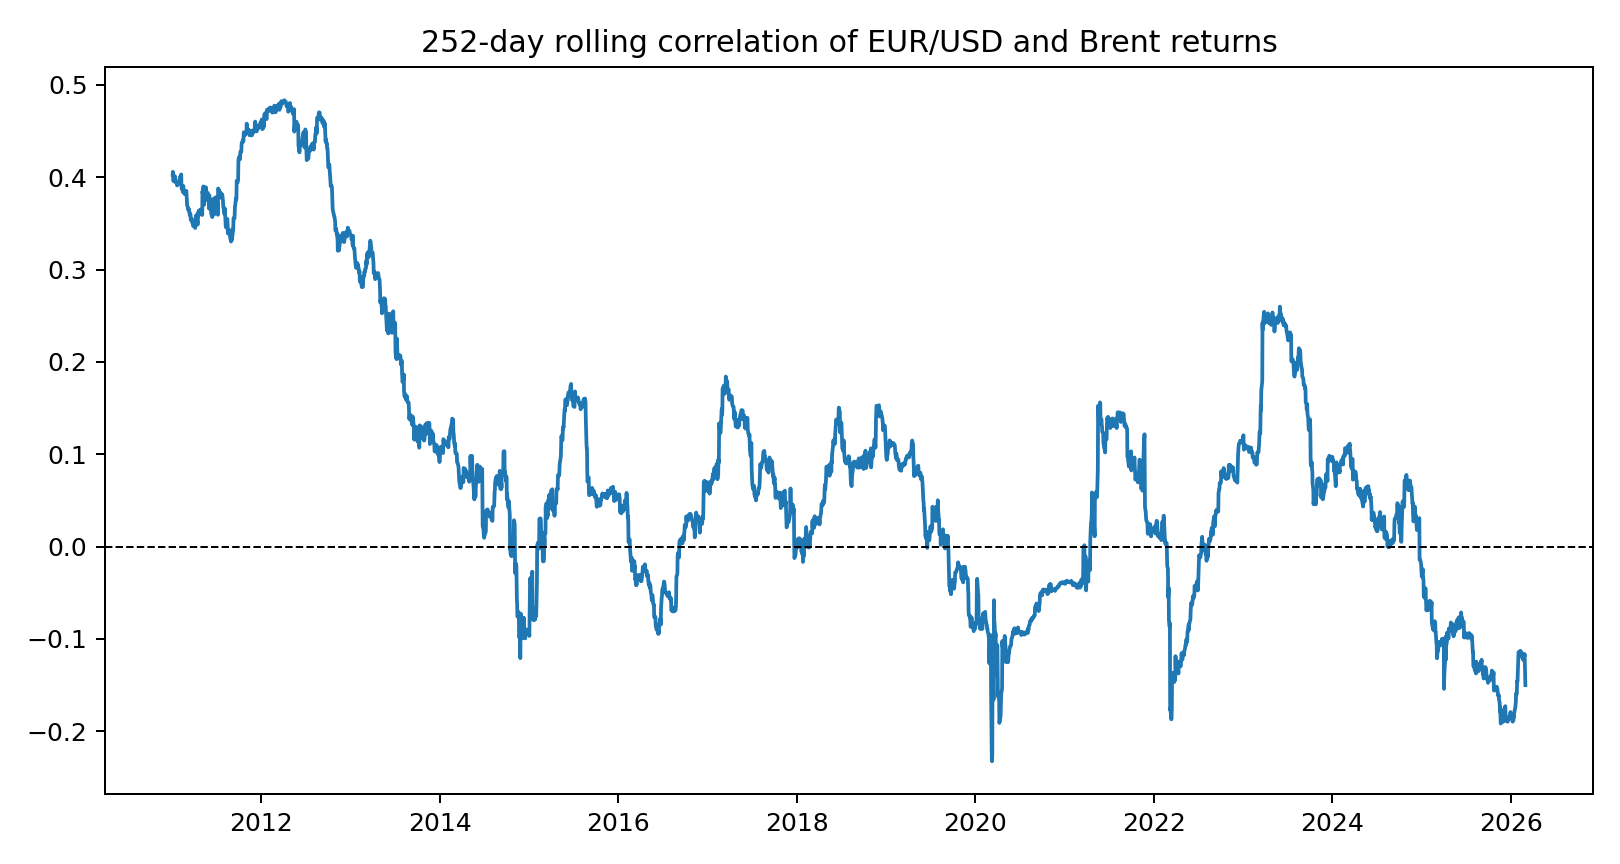
\includegraphics[width=0.85\textwidth]{results/rolling_correlation.png}
\caption{252-дневная скользящая корреляция}
\end{figure}

Это очень полезный график для устного рассказа. Он показывает, что корреляция плавает во времени. То есть связь не постоянная, а режимная. Это помогает связать мой результат со второй статьей ЕЦБ.

\section{Главные цифры, которые стоит помнить}
Ниже минимальный набор чисел, которые полезно держать в голове.

\begin{itemize}
    \item Полная дневная выборка: коэффициент при текущей доходности нефти примерно $0.014$, $p \approx 0.006$.
    \item До 2022 года: коэффициент примерно $0.016$, $p \approx 0.009$.
    \item После 2022 года: коэффициент примерно $0.004$, $p \approx 0.709$.
    \item Тест коинтеграции для 1999--2021: $p \approx 0.105$.
    \item Коэффициент ECM: примерно $-0.03$, $p \approx 0.071$.
\end{itemize}

\textbf{Как это переводить на русский язык.}
\begin{itemize}
    \item Краткосрочный эффект есть.
    \item Но он небольшой.
    \item И он нестабилен во времени.
    \item Долгосрочная связь выглядит намного слабее.
\end{itemize}

Когда я говорю ``значим'' или называю \textit{p-value}\footnote{\textit{p-value} --- вероятность получить настолько же сильный результат случайно, если на самом деле эффекта нет. Чем меньше \textit{p-value}, тем сильнее статистический аргумент в пользу эффекта.}, я имею в виду именно статистическую значимость результата.

\section{Что говорить на защите}

\subsection{Вариант рассказа на 3--5 минут}
\textbf{Шаг 1.} Тема проекта --- связь EUR/USD и нефти Brent.

\textbf{Шаг 2.} Литература говорит, что связь есть, но она может быть краткосрочной и зависеть от режима рынка.

\textbf{Шаг 3.} Я взял открытые данные FRED, чтобы проект был полностью воспроизводим.

\textbf{Шаг 4.} Для дневных данных я оценил регрессию доходностей, а для месячных данных проверил коинтеграцию и ECM.

\textbf{Шаг 5.} Получил, что рост нефти в среднем связан с ростом EUR/USD, то есть с относительным ослаблением доллара.

\textbf{Шаг 6.} Но после 2022 года эффект сильно ослабевает, а сильной долгосрочной причинности нет.

\textbf{Шаг 7.} Поэтому нефть можно использовать как дополнительный фактор валютного риска, но не как единственный инвестиционный сигнал.

\subsection{Если попросят объяснить совсем простыми словами}
Можно сказать так:

\begin{quote}
Я проверял, помогает ли нефть понимать движение EUR/USD. Оказалось, что раньше эта связь была заметнее, а в последние годы стала слабее. Поэтому нефть полезна как дополнительный индикатор, но строить на ней одной стратегию нельзя.
\end{quote}

\section{Какие вопросы могут задать и что отвечать}

\subsection{Почему именно EUR/USD и Brent?}
Потому что именно такая связка обсуждается в данных статьях, а Brent --- один из главных мировых нефтяных бенчмарков.

\subsection{Почему FRED, а не Yahoo Finance или другой источник?}
Потому что FRED открыт, стабилен и удобен для автоматической загрузки. Для учебного проекта это лучший вариант с точки зрения воспроизводимости.

\subsection{Почему ты разделил выборку на до 2022 и после 2022?}
Потому что статья 2025 года специально смотрит свежий пост-2022 период, а статья ЕЦБ подчеркивает, что связь зависит от режима рынка. Мне было важно проверить, не изменилась ли она в последние годы.

\subsection{Почему ты не делаешь сильный вывод о долгосрочной связи?}
Потому что статистика на моей выборке это не поддерживает достаточно уверенно. Коинтеграция пограничная, ECM тоже не сверхсильный. Лучше честный аккуратный вывод, чем натянутый.

\subsection{В чем практический смысл для инвестора?}
Нефть может быть полезным дополнительным сигналом для оценки валютного риска по доллару, но сама по себе не дает полноценной торговой стратегии.

\section{Итог для себя}
Если мне нужно запомнить проект одной фразой, то она такая:

\begin{quote}
Мой проект показывает, что между нефтью Brent и EUR/USD есть положительная краткосрочная связь, но она нестабильна во времени и заметно слабее в последние годы, поэтому нефть стоит использовать как дополнительный фактор, а не как единственный сигнал.
\end{quote}

Этого уже достаточно, чтобы уверенно рассказывать проект и отвечать на базовые вопросы.

\end{document}
